\documentclass{article}
\usepackage[utf8]{inputenc}
\usepackage{graphicx}
\graphicspath{{images/}}

\title{Part 2 Final Project}
\author{Daniel Ocampo and Jeremy Moore }
\date{November 2017}
\usepackage{graphicx}
\begin{document}

\maketitle

\section{Objective}

Progress report (3-4 pages) Deadline: Friday, 17 th November, 2017 by 2:30pm:
Describe everything you have done so far in your progress report. By this point, you should
have conducted necessary research on the background, examined in detail the data set you
have selected, decided on the approach you will use to analyze it, and made a significant
progress towards implementation. Describe anything new that you have learned so far and
any unexpected challenges that you have encountered.

\section{introduction}

One of the things that I we want to analyze,  is developing countries, but because there are so many developing countries we just decided to understand our country. One A key indicators for evaluating the health of a country is through GDP.  While The United states GDP is at 1.5 growth rate as a whole, we were wondering if could can look at certain areas considering the fact that the United States is the the 3rd biggest in the world, We figured it would be wise to look at GDP per capita. We hope to analyze data for from the GDP per capita from the year of 2016, because we want to see if any fiscal policies have affected economic growth. We would Also like to take into account monetary polices as well, to see if they have anything to do with wit economic growth. T

\section{Data}
\begin{figure}[ht!]
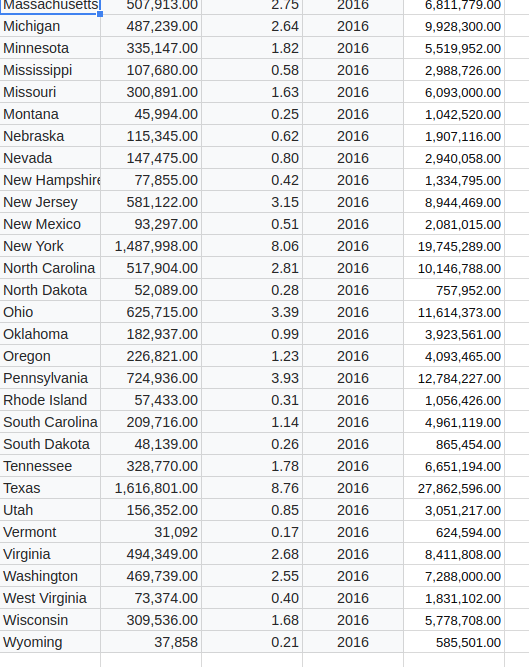
\includegraphics[width=15cm, height=15cm]{Data.png}
\caption{ Data For for GDP  }
\end{figure}
               



We currently only have a data set for one year, because we are having trouble figure out to calculate GDP based on the total amount a country as made. For the current Data  set we have the name of the state which is then listed below. The Next column is the amount of money we that state has produced. This ranges for sales inside the state. For Example, it would calculate the amount cars that we sold and produced there. The mount money spent on steal, food, services, and net exports. The next column tells us the pace that it is growing, so right now the state with largest growing GDP is California with 14\% growth rate. The next column that we have is the population size of the country. the next Column is the population size, which just tells the population size of the year of 2016. last relevant column that we have is the year column, this is just used to specify the year in which we have  

\section{Our Learning process}

So far based on looking at the data we can see that states with a higher population tend to have a higher GDP. Can the correlation between population be and GDP be concluded. Does it work for every state? there are many questions that need to be taken into consideration. One way that we can look at this is by making a a graph bar chart that list the the population size by the state and then making the color change based on the their GDP.  Another thing we can see is what states need attention, in regrades to GPD, what state has the lowest GDP, are they small state that it does it even matter, or are they big and utilizing their natural resource to their full capacity. Is their not enough incentive for entrepreneurs to take risks, is there to many taxes on that state. 


\section{Concerns}

one of our major concerns is that we should also take to account real GDP. While GDP  might be  high, we should I also take to account Real GDP which is adjusted for price changes. I guess one of our concerns is that If we to want to compare GDP with different years we would have to Real GDP for a given year, in relation to a "base" year. Which is computed by having a base year and then multiplying it by by the nominal GDP for that particular year( using the GDP Deflator).  





\end{document}